\documentclass[12pt]{article}
\usepackage[utf8]{inputenc}
\usepackage{amsmath}
\usepackage{graphicx}
\usepackage{array}
\usepackage{geometry}
\geometry{margin=2.5cm}
\usepackage{titlesec}
\usepackage{float}
\usepackage{grffile} % importante para nombres de archivo con puntos o caracteres especiales
\titleformat{\section}{\centering\bfseries\uppercase}{\thesection}{1em}{}

\begin{document}

\section*{ DISEÑO A FLEXIÓN DE VIGA 30X50 }

\begin{minipage}[t]{0.48\textwidth}
\begin{tabular}{|l|c|}
\hline
Base (b) &  m \\
Altura (h) &  m \\
Recubrimiento (r) &  m \\
Estribo (\ensuremath{\phi_e}) &  m \\
Varilla principal (\ensuremath{\phi_s}) &  m \\
f'c &  MPa \\
fy &  MPa \\
\hline
\end{tabular}
\end{minipage}
\hfill
\begin{minipage}[t]{0.48\textwidth}

\begin{figure}[H]
\centering
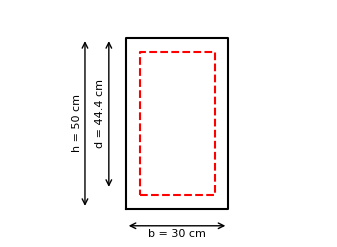
\includegraphics[height=5cm]{ section.png }
\end{figure}

\end{minipage}

\vspace{0.5cm}





\vspace{0.5cm}





\vspace{0.5cm}





\vspace{0.5cm}





\vspace{0.5cm}





\vspace{0.5cm}





\vspace{0.5cm}





\end{document}